\documentclass[t]{beamer}
\usetheme[deutsch]{KIT}
\setbeamercovered{transparent}
\setbeamertemplate{navigation symbols}{}

\KITfoot{Tutoriumsmaterial von Joachim Priesner, Sebastian Ullrich und Max Wagner \hspace{2.5cm} Basierend auf den Folien von Simon Stroh und Moritz v. Looz}
\usepackage[utf8]{inputenc}
\usepackage{amsmath}
\usepackage{ifthen}
\usepackage{amssymb}
\usepackage{tikz}
\usepackage{ngerman}
\usepackage[normalem]{ulem}
\usetikzlibrary{automata}
\usenavigationsymbols


\title{Theoretische Grundlagen der Informatik}
\subtitle{Tutorium}
\author{Moritz von Looz, Simon Stroh}

\institute[ITI]{Institut für Theoretische Informatik}

\TitleImage[height=\titleimageht]{images/tmaschine.png}

\newcommand{\N}{\ensuremath{\mathbb{N}}}
\newcommand{\M}{\ensuremath{\mathcal{M}}}
\newcommand{\classP}{\ensuremath{\mathcal{P}}}
\newcommand{\classNP}{\ensuremath{\mathcal{NP}}}
\newcommand{\co}{\ensuremath{\mathsf{co\text{-}}}}
\newcommand{\pot}{\ensuremath{\mathcal{P}}}
\newcommand{\abs}[1]{\ensuremath{\left\vert #1 \right\vert}}
\newcommand{\menge}[2]{\ensuremath{\left\lbrace #1 \,\middle\vert\, #2 \right\rbrace}}
\newcommand{\ducttape}[1]{\vspace{#1}}
\newcommand{\neglit}[1]{\overline{#1\vphantom{x^a}}}
\newcommand{\recipe}{\raisebox{-.3cm}{\includegraphics[scale=.15]{images/chefs-cap.png}}\hspace{0.2cm}}
\newcommand{\opt}[1]{\ensuremath{\text{OPT}(#1)}}
\newcommand{\A}[1]{\ensuremath{\mathcal{A}(#1)}}
\renewcommand{\O}[1]{\ensuremath{\mathcal{O}(#1)}}
\newcommand{\msout}[1]{\text{\sout{\ensuremath{#1}}}}

\newcommand{\invincible}{\setbeamercovered{invisible}} %  "Yesss! I am invincible!!" (Boris Grishenko)
\newcommand{\vincible}{\setbeamercovered{transparent}}
\renewcommand{\solution}[1]{\invincible \pause #1 \vincible}
\newcommand{\micropause}{\\[8pt]}

% \@ifundefined{tikzset}{}{\tikzset{initial text=}} % Text "start" bei Startknoten unterdrücken
\tikzstyle{every node}=[thick]
\tikzstyle{every line}=[thick]

\newcommand{\tutnr}[1]{
  \subtitle{Tutorium #1}
	\begin{frame}
		\maketitle
	\end{frame}
}

\newcommand{\uebnr}[1]{
  \subtitle{Anmerkungen zum #1. Übungsblatt}
	\begin{frame}
		\maketitle
	\end{frame}
}

\begin{document}

\newcommand{\start}[3]
{
  \draw (#1*2,#2*2) node{$#3$};
  \draw (#1*2,#2*2) circle(0.4cm);
  \draw [->] (#1*2-0.9,#2) -- (#1*2-0.4,#2);
}
\newcommand{\final}[3]
{
  \draw (#1*2,#2*2) node{$#3$};
  \draw (#1*2,#2*2) circle(0.4cm);
  \draw (#1*2,#2*2) circle(0.32cm);
}
\newcommand{\startfinal}[3]
{
  \draw (#1*2,#2*2) node{$#3$};
  \draw (#1*2,#2*2) circle(0.4cm);
  \draw (#1*2,#2*2) circle(0.32cm);
  \draw [->] (#1*2-0.9,#2) -- (#1*2-0.4,#2);
}
\newcommand{\state}[3]
{
  \draw (#1*2,#2*2) node{$#3$};
  \draw (#1*2,#2*2) circle(0.4cm);
}
\newcommand{\tol}[4]
{
  \draw (#1+#3,#2*2) node[above]{$#4$};
  \draw [->] (#1*2-0.4,#2*2) -- (#3*2+0.4,#2*2);
}
\newcommand{\tor}[4]
{
  \draw (#1+#3,#2*2) node[above]{$#4$};
  \draw [->] (#1*2+0.4,#2*2) -- (#3*2-0.4,#2*2);
}
\newcommand{\tot}[4]
{
  \draw (#1*2,#2+#3) node[right]{$#4$};
  \draw [->] (#1*2,#2*2+0.4) -- (#1*2,#3*2-0.4);
}
\newcommand{\tob}[4]
{
  \draw (#1*2,#2+#3) node[right]{$#4$};
  \draw [->] (#1*2,#2*2-0.4) -- (#1*2,#3*2+0.4);
}
\newcommand{\totl}[5]
{
  \draw (#1+#3,#2+#4) node[above right]{$#5$};
  \draw [->] (#1*2-0.283,#2*2+0.283) -- (#3*2+0.283,#4*2-0.283);
}
\newcommand{\totr}[5]
{
  \draw (#1+#3,#2+#4) node[above left]{$#5$};
  \draw [->] (#1*2+0.283,#2*2+0.283) -- (#3*2-0.283,#4*2-0.283);
}
\newcommand{\tobl}[5]
{
  \draw (#1+#3,#2+#4) node[below right]{$#5$};
  \draw [->] (#1*2-0.283,#2*2-0.283) -- (#3*2+0.283,#4*2+0.283);
}
\newcommand{\tobr}[5]
{
  \draw (#1+#3,#2+#4) node[below left]{$#5$};
  \draw [->] (#1*2+0.283,#2*2-0.283) -- (#3*2-0.283,#4*2+0.283);
}
\newcommand{\rloopl}[3]
{
  \draw (#1*2-1,#2*2) node[left]{$#3$};
  \draw [->] (#1*2-0.35,#2*2-0.2) arc (-30:-320:0.32cm);
}
\newcommand{\rloopr}[3]
{
  \draw (#1*2+1,#2*2) node[right]{$#3$};
  \draw [->] (#1*2+0.35,#2*2+0.2) arc (150:-140:0.32cm);
}
\newcommand{\rloopt}[3]
{
  \draw (#1*2,#2*2+1) node[above]{$#3$};
  \draw [->] (#1*2-0.2,#2*2+0.35) arc (240:-50:0.32cm);
}
\newcommand{\rloopb}[3]
{
  \draw (#1*2,#2*2-1) node[below]{$#3$};
  \draw [->] (#1*2+0.2,#2*2-0.35) arc (60:-230:0.32cm);
}
\newcommand{\lloopl}[3]
{
  \draw (#1*2-1,#2*2) node[left]{$#3$};
  \draw [->] (#1*2-0.35,#2*2+0.2) arc (30:320:0.32cm);
}
\newcommand{\lloopr}[3]
{
  \draw (#1*2+1,#2*2) node[right]{$#3$};
  \draw [->] (#1*2+0.35,#2*2-0.2) arc (-150:140:0.32cm);
}
\newcommand{\lloopt}[3]
{
  \draw (#1*2,#2*2+1) node[above]{$#3$};
  \draw [->] (#1*2+0.2,#2*2+0.35) arc (-60:230:0.32cm);
}
\newcommand{\lloopb}[3]
{
  \draw (#1*2,#2*2-1) node[below]{$#3$};
  \draw [->] (#1*2-0.2,#2*2-0.35) arc (-240:50:0.32cm);
}
\tutnr{5}

\section{Altlasten}
\subsection{CYK}
\begin{frame}
	\frametitle{CYK Darstellungen}
\end{frame}

\section{Turingmaschine}
\subsection{Allgemeine Turingmaschine}
\subsection{Turingmaschine}
\begin{frame}
	\frametitle{Turingmaschine}
	Die Turingmaschine besteht aus einem beidseitig \emph{unendlichen} Eingabe- und Rechenband
	mit einem frei beweglichen Lese-/Schreibkopf, der von einer \emph{endlichen} Kontrolle gesteuert wird. 
	\begin{center}
		\includegraphics[scale=0.5]{images/tmaschine.png}
	\end{center}
\end{frame}
\begin{frame}
\frametitle{Turingmaschine}
\begin{block}{Definiton}
Eine Turingmaschine wird definiert als ein 7-Tupel bestehend aus:
 \begin{itemize}
 \item $Q$, einer endlichen Zustandsmenge
 \item $\Sigma$, einem endlichen Eingabealphabet
 \item $\sqcup$, einem Blanksymbol mit $\sqcup \notin \Sigma$
 \item $\Gamma$, einem endlichen Bandalphabet mit $\Sigma \cup\{\sqcup\} \subseteq \Gamma$
 \item $s \in Q$, einem Startzustand
 \item $\delta$, einer Übergangsfunktion $\delta: Q\times\Gamma \rightarrow Q\times\Gamma\times\{L, R, N\}$
 \item $F \subseteq Q$, einer Menge an Endzuständen
 \end{itemize}
\end{block}
\begin{block}{Bemerkung}
 Für $q\in F$ gilt: $\forall a \in \Gamma: \delta(q, a) = (q, a, N)$, d.h. die Berechnung der Turingmaschine stoppt.
\end{block}
\end{frame}

\frame{
	\frametitle{Graph einer Turingmaschine}
	\begin{center}
	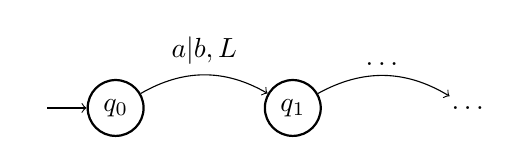
\begin{tikzpicture}[node distance=2.25cm,auto]
	\node(q0)[draw,circle,thick]{$q_0$};
	\node (s) [node distance=1cm,left of =q0]{};
	\node(q1)[draw,circle,thick,right of=q0]{$q_1$};
	\node(qx)[right of=q1]{\dots};

	\path[->]       (s) edge (q0)
	                (q0) edge[bend left] node{$a|b,L$} (q1)
			                (q1) edge[bend left] node{\dots} (qx);
					\end{tikzpicture}
					\end{center}

					Dabei steht die Kantenbeschriftung "`$a|b,L$"' für den Übergang $\delta(q_0,a) =
					(q_1,b,L)$.

					\vspace{2mm}
					Falls es für einen gegebenen Zustand und ein gegebenes
					Symbol keinen Zustandsübergang gibt, bricht die Maschine die Berechnung ab. 
}

\begin{frame}
	\frametitle{Turingmaschine: Beispiel}

	Seien $\Sigma = \{0,1\}$, $\Gamma = \{0,1,\sqcup\}$ und die Turingmaschine $\M =(\{q_0, q_1,q_2,q_f\},\Sigma, \sqcup, \Gamma,\delta,q_0,\{q_f\})$ mit folgender Überführungsfunktion gegeben:

	\begin{center}
	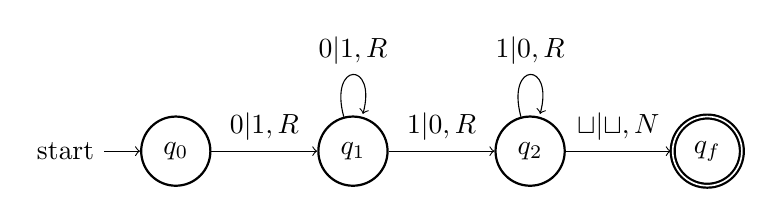
\begin{tikzpicture}[node distance=2.25cm,auto]
	\node(q0)[state,initial]{$q_0$};
	\node(q1)[state,right of=q0]{$q_1$};	
	\node(q2)[state,right of=q1]{$q_2$};	
	\node(qf)[state,accepting,right of=q2]{$q_f$};	

	\path[->]       (q0) edge node{$0|1,R$} (q1)
					(q1) edge node{$1|0,R$} (q2)
	                (q1) edge[loop above] node{$0|1,R$} (q1)	                
			        (q2) edge[loop above] node{$1|0,R$} (q2)
			        (q2) edge node{$\sqcup|\sqcup,N$} (qf);
					\end{tikzpicture}
					\end{center} 

	\begin{itemize}
		\item Welche Wörter akzeptiert \M{}?
		\item Wie verändert \M{} die Eingabe?
	\end{itemize}			
\end{frame}


\begin{frame}
\frametitle{Konfigurationen}
Sei $\mathcal{M} =(Q,\Sigma, \sqcup, \Gamma,\delta,s,F)$ eine Turingmaschine.

Angabe des aktuellen Berechnungszustandes: \emph{Konfiguration}

$$w(q)av$$ 

wobei $w,v \in \Gamma^*, a \in \Gamma$ und $q\in Q$. \\

Dies bedeutet:

\begin{itemize}
	\item $\mathcal{M}$ befindet sich im Zustand $q$.
	\item Der Lesekopf steht auf dem Zeichen $a$.
	\item Links vom Lesekopf steht das Wort $w$ und rechts davon das Wort $v$ auf dem Rechenband.
\end{itemize}
\end{frame}

\subsection{Linear platzbeschränkte Turingmaschine}
\begin{frame}
	\frametitle{Linear platzbeschränkte Turingmaschine}
	TODO
\end{frame}

\section{Schluss}
\subsection{Schluss}

\begin{frame}
\frametitle{Bis zum nächsten Mal!}
\begin{center}
  \includegraphics[width=1 \textheight]{images/xkcd_205.png}
\end{center}
\end{frame}

\input{includes/disclaimer}
\end{document}